\documentclass[12pt]{article}

\usepackage[T1]{fontenc}
\usepackage{mathptmx}
\usepackage{fancyvrb}

\topmargin 0.0in
\setlength{\textwidth} {420pt}
\setlength{\textheight} {620pt} 
\setlength{\oddsidemargin} {20pt}
\setlength{\marginparwidth} {72in}

\usepackage{fancyhdr} 
\usepackage{url}

% set it so that subsubsections have numbers and they
% are displayed in the TOC (maybe hard to read, might want to disable)

\setcounter{secnumdepth}{3}
\setcounter{tocdepth}{3}

% define widow protection

\def\widow#1{\vskip #1\vbadness10000\penalty-200\vskip-#1}

\clubpenalty=10000  % Don't allow orphans
\widowpenalty=10000 % Don't allow widows

% this should give me the ability to use some math symbols that 
% were available by default in standard latex (i.e. \Box)

\usepackage{latexsym}
\usepackage{graphicx}
\usepackage{listings}

% define a little section heading that doesn't go with any number

\def\littlesection#1{
\widow{2cm}
\vskip 0.5cm
\noindent{\bf #1}
\vskip 0.0001cm 
}

\pagestyle{fancyplain}

\newcommand{\tstamp}{\today}   
\renewcommand{\sectionmark}[1]{\markright{#1}}
\lhead[\Section \thesection]            {\fancyplain{}{\rightmark}}
\chead[\fancyplain{}{}]                 {\fancyplain{}{}}
\rhead[\fancyplain{}{\rightmark}]       {\fancyplain{}{\thepage}}
\cfoot[\fancyplain{\thepage}{}]         {\fancyplain{\thepage}{}}

\newlength{\myVSpace}% the height of the box
\setlength{\myVSpace}{1ex}% the default, 
\newcommand\xstrut{\raisebox{-.5\myVSpace}% symmetric behaviour, 
  {\rule{0pt}{\myVSpace}}%
}

% leave things with no spacing extra spacing in the final version of the paper
\renewcommand{\baselinestretch}{1.0}    % must go before the begin of doc

% suppress the use of indentation for a paragraph

\setlength{\parindent}{0.0in}
\setlength{\parskip}{0.1in}

\begin{document}

%% \begin{abstract}

%%   Try

%% \end{abstract}

% handle widows appropriately
\def\widow#1{\vskip #1\vbadness10000\penalty-200\vskip-#1}

% build the title section

\makeatletter

\def\maketitle{%
  %\null
  \thispagestyle{empty}%
  %\vfill
  \begin{center}%\leavevmode
    %\normalfont
% define a little s
    {\Huge \@title\par}%
    %\hrulefill\par
    \vspace*{.1in}
    {\normalsize \@author\par}%
    \vskip .1in
%    {\Large \@date\par}%
  \end{center}%
  %\vfill
  %\null
  %\cleardoublepage

  }

\makeatother

\vspace*{-1.1in}
\title{Lab 7 Group 4}
\vspace*{-.1in}
% build the author section
\author{Kara King, Dibyajyoti Mukherjee, Eric Weyant, Shane Regel, Andreas Landgrebe\\
Department of Computer Science\\
Allegheny College \\
\vspace*{.2in} \today \\ \vspace*{.2in}
{\bf Abstract} \\ A document containing each of the eight deliverables for laboratory 7.}

% use the default title stuff
\maketitle

\vspace*{.1in}
\section{Member Contributions and Tool Support}
\label{sec:one}
\vspace*{-.1in}
\subsection{Member Contributions}
\textbf{Andreas Landgrebe:}
Printed the output for Deliverable 5.
Description of the output made from running the run.sh script for Deliverable 6.

\textbf{Kara King:}
Description of the the target in the build.xml and order for mutation for Deliverable 2.
Listing of the steps for the Demonstration of MAJOR for Deliverable 8.

\textbf{Dibyajyoti Mukherjee:}
Extra Credit to explain how to use MAJOR to perform mutation analysis on ReleasePlanner project to make sure that this demo of MAJOR will work properly.
Maintained build.xml file in order to run with the main method and also run MAJOR with ReleasePlanner.

\textbf{Eric Weyant:}
Write a main method in Triangle.java for demonstration purposes for Deliverable 3. 
Print the output from running Triangle.java with the modified main verision for Deliverable 4.

\textbf{Shane Regel:}
Thoughtful commentary on one live and one killed source code mutant for Deliverable 7.
Converted deliverables into LaTeX.

\subsection{Tools}

\textbf{Gvim:} Gvim was used to create the main method and also analyze the Triangle.java program.

\textbf{LaTeX(Texmaker):} Texmaker was used to compile LaTeX code for each deliverable.

\textbf{BitBucket:} Bitbucket was used via Git commands so we were able to maintain version control throughout the lab.

\textbf{Major Mutation System:} Major was used for mutation analysis of the Triangle project in conjunction with the Ant build system. 

\textbf{Apache Ant:} Ant is used with our group$’$s build.xml file to run our entire project alongside in conjunction with other tools such as MAJOR.
\vspace*{.1in}
\section{Description of targets in the build.xml and the order in which they are run}
\label{sec:two}
\vspace*{-.1in}
There are many targets within the build.xml file for this project. The first target is clean. This target simply cleans up the files by eliminating the bin directory, which is the directory that holds all of the compiled code, along with the .csv and .log files. The next target is init. This target simply initializes the build for the project by creating the bin directory. The next target is compile. This target compiles all of the source files in the src directory and then puts the compiled versions in the bin directory. This target depends on the init target. Also, this target adapts to use Major's compiler and it must pass the mml script to Major's compiler. It then generates mutants in the projects code and outputs a .log file that shows a description of all the mutants created. The next target is compile.tests. This target compiles all of the source code in the test directory and puts all the compiled versions in the bin directory. This target depends on the compile target. Also, this target executes the javac file executable. The next target is mutation.test. This target is the adapted mutation test target that uses Major's junit task. Essentially, this target is used to run the mutation analysis for the the test cases in our project. The results of this target go into the kill.csv file. This file tells the programmer how many mutants were alive and how many failed after this target is run. The main output from this target being run is put into the results.csv file which shows a summary of the time took to run coverage, how much our tests covered, how many mutants were kills versus how many were not, and a few other details. This target does this since the mutationAnalysis attribute is set to true. The next target is run. This target simply runs the Triangle classes main method and produces the output the main method lays out. The final target is test. This target runs all of the test files and prints out the summary of the tests such as whether they passed, failed, how long they took, and how many tests there were that ran.


The order of commands that are executed during mutation are as followed.
The first step is ant -Dmutation="=../mml/tutorial.mml.bin\" which sets the path the the mml file we are using.  Then, an ant clean command is done in order to get rid of the already existing bin directory from the previous trial run. Next, the build is initialized from the ant init command, however, if one simply runs ant compile or ant compile.tests after a clean, this will build the bin directory. Hence, if those commands are used, the ant init command does not have to be typed out. Once the bin directory is made, or in other words the build is initialized, the ant compile command is run which puts mutants into  the code and compiles the src directory. Then,  ant compile.tests is ran which compiles all the tests and puts their compile code into the bin directory. Then, during the process, ant test is run to see how good the tests do without the mutation analysis. The final step is running ant mutation.test which runs the tests using mutation. These commands should be run in this order for mutation to ensure that the major compiler is bound to the java compiler to ensure that mutants are added into the code before the actual testing of the test suite using mutation analysis is done. We must set the path to the mml file before anything is done so the program knows what compiler and jar file to use. Mutation analysis is the last step because the programmer needs to make sure their test suite compiles correctly before they can run mutation analysis on the tests.  
\vspace*{.1in}
\section{Modified Main}
\label{sec:three}
See attatched programs
\vspace*{.1in}
\section{Output from running Triangle.java with main}
\label{sec:four}
\vspace*{-.1in}
\lstinputlisting[basicstyle=\ttfamily\scriptsize, float=h,frame=tb,caption=Main output,label=zebra]{mainoutput.txt}
\vspace*{.1in}
\section{Output from executing run.sh}
\label{sec:five}
\vspace*{-.1in}
\VerbatimInput{runoutput.txt}

\vspace*{.1in}
\section{Analysis of Output from run.sh}
\label{sec:six}
\vspace*{-.1in}

In the output produced by the run.sh script, all of the four compilations of ant comands built successfully. These four compilation of ant commands are in the run.sh file.  On the first part of the run.sh script, the project is being tested if it is compiling and mutating. In this example.

During this first part, the bin directory is being cleared and deleted, then it will create another bin directory where all of the compiled source code is stored. After this, it will compile the source code and check if the source code builds correctly. Then it will generate the mutants and put them into the byte code of the source code along with creating a mutants.log files that gives a representation of all the mutants that were created and put into the source code. This part also outputs into the terminal that there were 79 mutants made with 21 ms. This first set of commands in the script has a command that also specifies that the compiling process should include mutation using the MML script in our project.

The next set of ant commands in the script file compiles the test source code to see if they build correctly. From the output shown, the test cases were successfully compiled and the build was successful which took 1 second in total. This set of commands puts all of the compiled source code from the tests folder in the bin directory. 

After this, the script file will run the tests without mutation analysis, which is the same as running the command ant test. From this, it will now go through the build file and go through each junit test that was written. In the output, each junit test, will display the test cases and show how much time it took for the test cases to be run. At the top of the output from the run.sh file, it shows the number of tests being run, the number of failures, the number of errors, and how long it took for all of the test to be run. At the bottom of the screen, it will show that the build was successful and total time was 0 second.

The last set of ant commands in the script runs the tests with mutation analysis. As shown in the output, the junit testing will have the mutation analysis enabled and this analysis will show a number of key information. The first number will show how many ordered tests will run to verify independency. After this, the mutation analysis will display the amount of time it took to preprocess the mutation analysis, which in our case was 0.09 seconds. After that, the next number being displayed is the number of mutants that is being covered, which was 79. After this, it will display how long it takes to run the test suites, which in our case took 22 milliseconds. Then it will show the total time it has taken so far to run the tests cases along with the number of mutants that were covered in total. From this, it will show the number of mutants that was killed and how many that was currently alive after running the test cases.  As shown in the output, there are 70 mutants that are killed and 9 that are currently alive in the source code. After this, it displays the total summary from running the test cases using the mutation analysis. This summary includes the total run time with the mutation analysis, the percentage of mutants that were killed over the amount that were still alive (the mutation score in this case was 88.61 percent). After this, the result of the test cases will now export the runtime results to results.csv and the mutant kill details to kill.csv. 

\vspace*{.1in}
\section{Live vs Killed Commentary}
\label{sec:seven}
\vspace*{-.1in}

\begin{figure}[p]
\centering
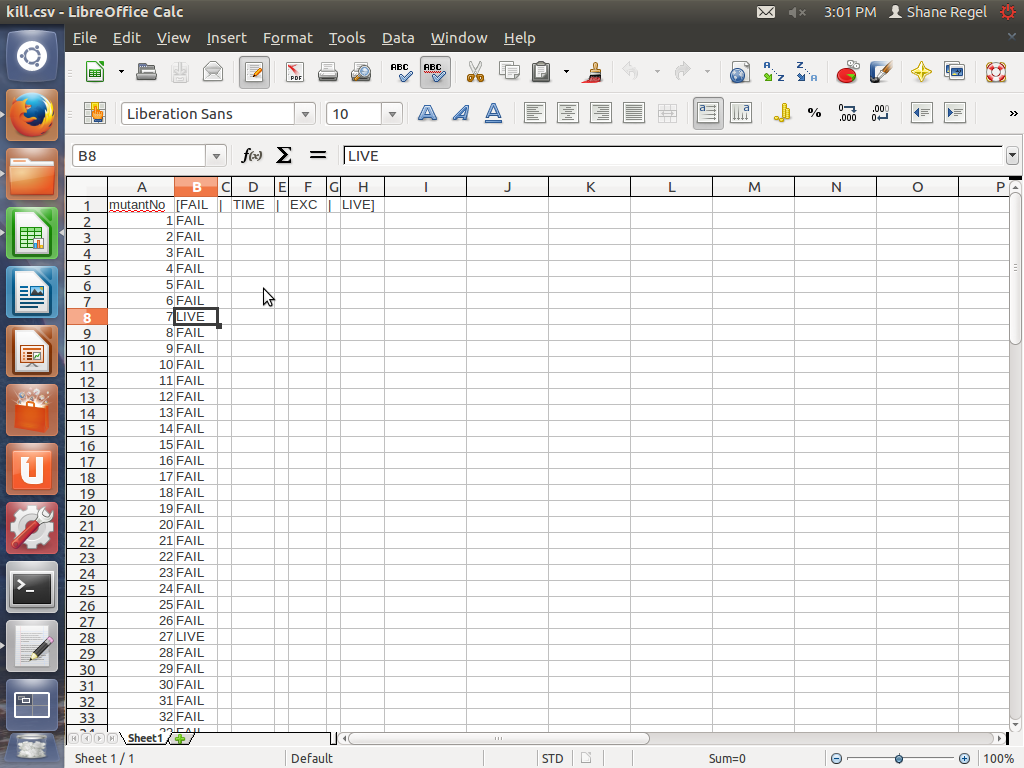
\includegraphics[width=0.8\textwidth]{Lab7Killcsv.png}
\caption{kill.csv File}
\label{fig:kill}
\end{figure}

\begin{figure}[p]
\centering
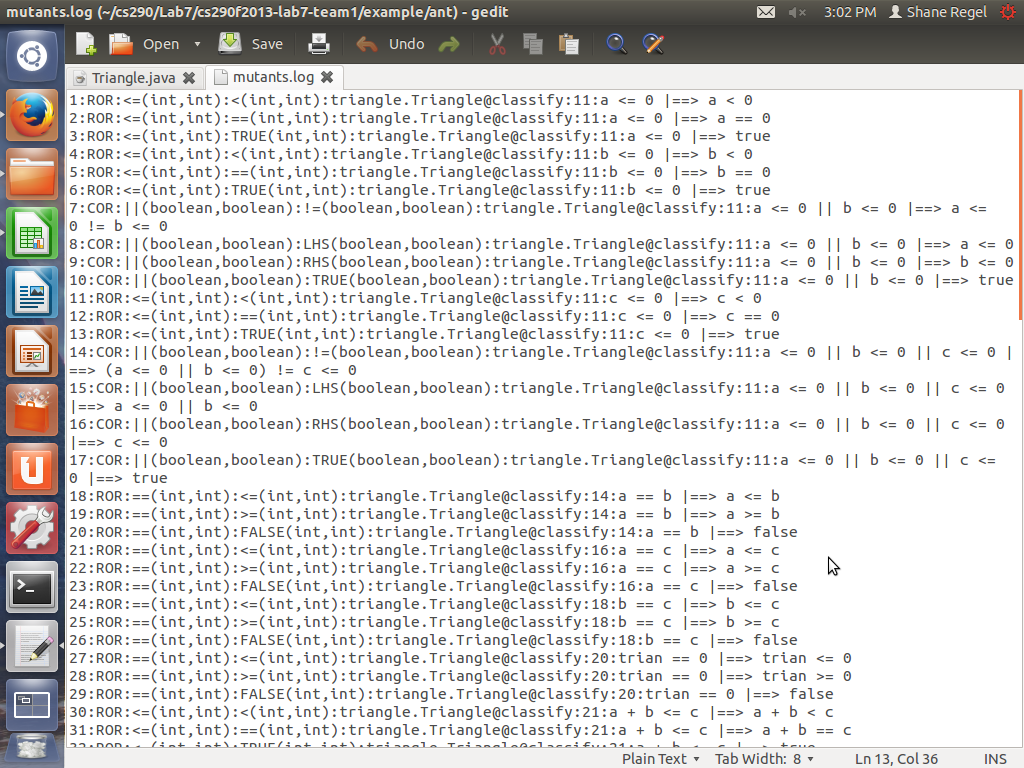
\includegraphics[width=0.8\textwidth]{Lab7mutationslog.png}
\caption{mutants.log File}
\label{fig:mutants}
\end{figure}

The kill.csv file provides information on whether or not the mutant was killed by the test cases. A mutant with the FAIL annotation is considered killed while one with the LIVE annotation remained alive after running the test cases. Figure~\ref{fig:kill} provides an example where mutant 6 was killed while mutant 7 remains alive. The log file, demonstrated in Figure~\ref{fig:mutants}, provides detailed information on each generated and embedded mutant. The file contains seven columns separated by a :, each of which represents a different piece of information on the mutant. The columns, in order, provide information on:

\begin{enumerate}
\item{Mutants unique number (id)}
\item{Name of the applied mutation operator}
\item{Original operator symbol}
\item{Replacement operator symbol}
\item{Fully qualified name of the mutated method}
\item{Line number in the original source file}
\item{Visualization of the applied transformation}
\end{enumerate}

For example mutant 6 (shown as two lines):\\

\begin{small}
\begin{lstlisting}
6:ROR:<=(int,int):TRUE(int,int):triangle.Triangle@classify: 
\end{lstlisting}
\begin{lstlisting}
11:b <= 0 |==> true
\end{lstlisting}
\end{small}

The mutant id is 6 and the mutation operator is ROR, which stands for relational operator replacement. The original operator was (int,int) and has been changed to TRUE(int,int). This mutation occurs in the classify method of Triangle on line 11. The operation b <= 0 has been replaced with true. This mutation was killed so the test cases were able to identify the replaced relational operator.

\par This mutation can be detected with a psuedo test case:\\

\begin{lstlisting}
b = 2; 
expected = if(b>0) => false 
           else => true  
actual = return value from method 
check (expected == actual) 
\end{lstlisting}
        
The psuedo code goes through the logic of a test case that finds the mutation. Initially b is set to 2. Then the case checks if b is greater than 0, which 2 is, so expected would be set to false. Actual finds the return value of the method in question. The mutation sets this value to true. Then the expected and actual values are compared, since they are not equal the test case fails and discovers the mutant.

\par The test cases were not able to identify mutant 7 (shown as two lines):\\ 

\begin{small}
\begin{lstlisting}
7:COR:||(boolean,boolean):!=(boolean,boolean):
\end{lstlisting}  
\begin{lstlisting}
triangle.Triangle@classify:11:a <= 0 || b <= 0 |==> a <= 0 != b <= 0
\end{lstlisting}
\end{small}

The id number is seven and the mutation operator is COR, which stands for conditional operator replacement. The original operator was (boolean,boolean) but has been changed to !=(boolean,boolean). This mutation occurs in the classify method of Triangle on line 11. The mutation changed the source code from a <= 0 || b <= 0 (a less than or equal to zero and b less than or equal to zero) to a <= 0 != b <= 0 (a less than or equal to zero not equal to b less than or equal to zero). The || (or) is changed to != (not equal to).


\par The test cases do not catch this error because the two statements are semantically equivalent. The difference between the two statements though can be seen in Truth Tables ~\ref{or} and ~\ref{notequal}.


\begin{table}[htbp]
\centering
\begin{tabular}{|c||c|c|}
\hline
\bf & \bf \textbf{||} & \bf \\\hline\hline
 & \textbf{T} & \textbf{F}\\\hline
\textbf{T} & T & T\\\hline
\textbf{F} & T & F\\\hline
\end{tabular}
\caption{OR}
\label{or}
\end{table}

\begin{table}[htbp]
\centering
\begin{tabular}{|c||c|c|}
\hline
\bf & \bf \textbf{!=} & \bf \\\hline\hline
 & \textbf{T} & \textbf{F}\\\hline
\textbf{T} & F & T\\\hline
\textbf{F} & T & F\\\hline
\end{tabular}
\caption{NOT EQUAL}
\label{notequal}
\end{table}

The instance that would pass the test case but be incorrect would be the true true instance for the != truth table. Specifically it avoids the statement:
\begin{lstlisting}
if (a <= 0 || b <= 0 || c <= 0)
           return Type.INVALID;
\end{lstlisting}
The mutant changes the statement to:
\begin{lstlisting}
if (a <= 0 != b <= 0 || c <= 0)
           return Type.INVALID;
\end{lstlisting}
In this case with the input (0, 0, 4) a = 0 and b = 0 so both statements evaluate to true, however since they are joined by a != they evaluate to false. Since c = 4 which is <= 0 the entire if returns false and the return invalid is never invoked. The issue is, (0, 0, 4) would not print out that the triangle is invalid due to having a side of 0.  The error is eventually discovered in the code with the statement:
\begin{lstlisting}
if (a + b <= c || a + c <= b || b + c <= a)
				return Type.INVALID;
\end{lstlisting}
Since 0+0<=4 the statement returns true and the return invalid is invoked.

\vspace*{.1in}
\section{Steps For Demonstration}
\label{sec:eight}
\vspace*{-.1in}

\begin{enumerate}
\item{Go into correct directory ../lab7/cs290f2013-lab7-team1/example/ant}
\item{Run the command ./run.sh}
\item{ Explain the commands that run.sh file calls and in the order they are called.
\begin{enumerate}
\item{ ant -Dmutation="=../mml/tutorial.mml.bin" clean compile}
\item{ant compile.tests}
\item{ ant test}
\item{ant mutation.test}
\end{enumerate}}
\item{Explain what each command produced
\begin{enumerate}
\item{ created bin directory and compiled the source code and put them into the bin directory along 
	    with adding in 79 mutants and a .log file of all the mutants. }
\item{compiles all of the tests and puts them into the bin directory}
\item{ This runs all of the tests and outputs how many tests ran, the amount that failed and errors that 	    occurred. It also shows the total time it took for the tests along with the time it took for each 	  	  test to complete.}
\item{ Runs the mutation analysis on the project and outputs the results into the terminal along with 	 	    creating a results.csv and kill.csv file}
\end{enumerate}}
\item{Go into the result files along with the terminal output and explain what each means.}
\end{enumerate}
\end{document}


